% Created by tikzDevice version 0.12.3.1 on 2021-12-15 12:29:49
% !TEX encoding = UTF-8 Unicode
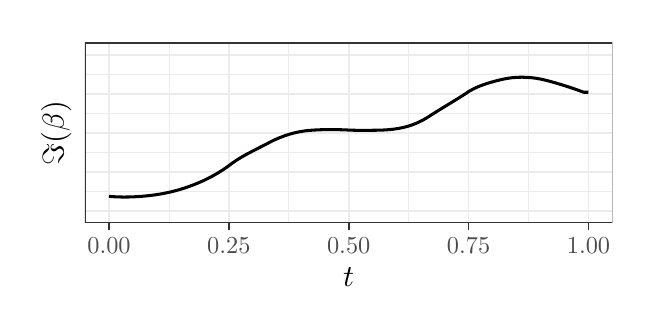
\begin{tikzpicture}[x=1pt,y=1pt]
\definecolor{fillColor}{RGB}{255,255,255}
\path[use as bounding box,fill=fillColor,fill opacity=0.00] (0,0) rectangle (216.81,101.18);
\begin{scope}
\path[clip] (  0.00,  0.00) rectangle (216.81,101.18);
\definecolor{drawColor}{RGB}{255,255,255}
\definecolor{fillColor}{RGB}{255,255,255}

\path[draw=drawColor,line width= 0.6pt,line join=round,line cap=round,fill=fillColor] (  0.00,  0.00) rectangle (216.81,101.18);
\end{scope}
\begin{scope}
\path[clip] ( 20.71, 30.69) rectangle (211.31, 95.68);
\definecolor{fillColor}{RGB}{255,255,255}

\path[fill=fillColor] ( 20.71, 30.69) rectangle (211.31, 95.68);
\definecolor{drawColor}{gray}{0.92}

\path[draw=drawColor,line width= 0.3pt,line join=round] ( 20.71, 42.08) --
	(211.31, 42.08);

\path[draw=drawColor,line width= 0.3pt,line join=round] ( 20.71, 56.15) --
	(211.31, 56.15);

\path[draw=drawColor,line width= 0.3pt,line join=round] ( 20.71, 70.22) --
	(211.31, 70.22);

\path[draw=drawColor,line width= 0.3pt,line join=round] ( 20.71, 84.28) --
	(211.31, 84.28);

\path[draw=drawColor,line width= 0.3pt,line join=round] ( 51.04, 30.69) --
	( 51.04, 95.68);

\path[draw=drawColor,line width= 0.3pt,line join=round] ( 94.35, 30.69) --
	( 94.35, 95.68);

\path[draw=drawColor,line width= 0.3pt,line join=round] (137.67, 30.69) --
	(137.67, 95.68);

\path[draw=drawColor,line width= 0.3pt,line join=round] (180.99, 30.69) --
	(180.99, 95.68);

\path[draw=drawColor,line width= 0.6pt,line join=round] ( 20.71, 35.05) --
	(211.31, 35.05);

\path[draw=drawColor,line width= 0.6pt,line join=round] ( 20.71, 49.11) --
	(211.31, 49.11);

\path[draw=drawColor,line width= 0.6pt,line join=round] ( 20.71, 63.18) --
	(211.31, 63.18);

\path[draw=drawColor,line width= 0.6pt,line join=round] ( 20.71, 77.25) --
	(211.31, 77.25);

\path[draw=drawColor,line width= 0.6pt,line join=round] ( 20.71, 91.32) --
	(211.31, 91.32);

\path[draw=drawColor,line width= 0.6pt,line join=round] ( 29.38, 30.69) --
	( 29.38, 95.68);

\path[draw=drawColor,line width= 0.6pt,line join=round] ( 72.69, 30.69) --
	( 72.69, 95.68);

\path[draw=drawColor,line width= 0.6pt,line join=round] (116.01, 30.69) --
	(116.01, 95.68);

\path[draw=drawColor,line width= 0.6pt,line join=round] (159.33, 30.69) --
	(159.33, 95.68);

\path[draw=drawColor,line width= 0.6pt,line join=round] (202.65, 30.69) --
	(202.65, 95.68);
\definecolor{drawColor}{RGB}{0,0,0}

\path[draw=drawColor,line width= 1.1pt,line join=round] ( 29.38, 40.23) --
	( 31.09, 40.10) --
	( 32.81, 40.02) --
	( 34.52, 39.98) --
	( 36.24, 39.99) --
	( 37.96, 40.04) --
	( 39.67, 40.13) --
	( 41.39, 40.25) --
	( 43.10, 40.41) --
	( 44.82, 40.60) --
	( 46.53, 40.84) --
	( 48.25, 41.12) --
	( 49.96, 41.45) --
	( 51.68, 41.83) --
	( 53.40, 42.26) --
	( 55.11, 42.74) --
	( 56.83, 43.27) --
	( 58.54, 43.87) --
	( 60.26, 44.52) --
	( 61.97, 45.22) --
	( 63.69, 45.99) --
	( 65.40, 46.83) --
	( 67.12, 47.74) --
	( 68.84, 48.73) --
	( 70.55, 49.81) --
	( 72.27, 50.99) --
	( 73.98, 52.28) --
	( 75.70, 53.44) --
	( 77.41, 54.48) --
	( 79.13, 55.45) --
	( 80.84, 56.35) --
	( 82.56, 57.23) --
	( 84.27, 58.11) --
	( 85.99, 58.99) --
	( 87.71, 59.89) --
	( 89.42, 60.73) --
	( 91.14, 61.46) --
	( 92.85, 62.11) --
	( 94.57, 62.67) --
	( 96.28, 63.14) --
	( 98.00, 63.52) --
	( 99.71, 63.82) --
	(101.43, 64.03) --
	(103.15, 64.16) --
	(104.86, 64.25) --
	(106.58, 64.32) --
	(108.29, 64.35) --
	(110.01, 64.35) --
	(111.72, 64.33) --
	(113.44, 64.29) --
	(115.15, 64.22) --
	(116.87, 64.14) --
	(118.59, 64.10) --
	(120.30, 64.09) --
	(122.02, 64.09) --
	(123.73, 64.10) --
	(125.45, 64.11) --
	(127.16, 64.14) --
	(128.88, 64.21) --
	(130.59, 64.33) --
	(132.31, 64.51) --
	(134.03, 64.77) --
	(135.74, 65.12) --
	(137.46, 65.57) --
	(139.17, 66.14) --
	(140.89, 66.84) --
	(142.60, 67.67) --
	(144.32, 68.66) --
	(146.03, 69.76) --
	(147.75, 70.84) --
	(149.47, 71.90) --
	(151.18, 72.95) --
	(152.90, 74.00) --
	(154.61, 75.05) --
	(156.33, 76.12) --
	(158.04, 77.21) --
	(159.76, 78.34) --
	(161.47, 79.26) --
	(163.19, 80.02) --
	(164.90, 80.65) --
	(166.62, 81.21) --
	(168.34, 81.71) --
	(170.05, 82.16) --
	(171.77, 82.56) --
	(173.48, 82.88) --
	(175.20, 83.11) --
	(176.91, 83.24) --
	(178.63, 83.28) --
	(180.34, 83.23) --
	(182.06, 83.10) --
	(183.78, 82.88) --
	(185.49, 82.57) --
	(187.21, 82.18) --
	(188.92, 81.73) --
	(190.64, 81.25) --
	(192.35, 80.74) --
	(194.07, 80.21) --
	(195.78, 79.66) --
	(197.50, 79.08) --
	(199.22, 78.47) --
	(200.93, 77.84) --
	(202.65, 77.84);
\definecolor{drawColor}{gray}{0.20}

\path[draw=drawColor,line width= 0.6pt,line join=round,line cap=round] ( 20.71, 30.69) rectangle (211.31, 95.68);
\end{scope}
\begin{scope}
\path[clip] (  0.00,  0.00) rectangle (216.81,101.18);
\definecolor{drawColor}{gray}{0.20}

\path[draw=drawColor,line width= 0.6pt,line join=round] ( 29.38, 27.94) --
	( 29.38, 30.69);

\path[draw=drawColor,line width= 0.6pt,line join=round] ( 72.69, 27.94) --
	( 72.69, 30.69);

\path[draw=drawColor,line width= 0.6pt,line join=round] (116.01, 27.94) --
	(116.01, 30.69);

\path[draw=drawColor,line width= 0.6pt,line join=round] (159.33, 27.94) --
	(159.33, 30.69);

\path[draw=drawColor,line width= 0.6pt,line join=round] (202.65, 27.94) --
	(202.65, 30.69);
\end{scope}
\begin{scope}
\path[clip] (  0.00,  0.00) rectangle (216.81,101.18);
\definecolor{drawColor}{gray}{0.30}

\node[text=drawColor,anchor=base,inner sep=0pt, outer sep=0pt, scale=  0.88] at ( 29.38, 19.68) {0.00};

\node[text=drawColor,anchor=base,inner sep=0pt, outer sep=0pt, scale=  0.88] at ( 72.69, 19.68) {0.25};

\node[text=drawColor,anchor=base,inner sep=0pt, outer sep=0pt, scale=  0.88] at (116.01, 19.68) {0.50};

\node[text=drawColor,anchor=base,inner sep=0pt, outer sep=0pt, scale=  0.88] at (159.33, 19.68) {0.75};

\node[text=drawColor,anchor=base,inner sep=0pt, outer sep=0pt, scale=  0.88] at (202.65, 19.68) {1.00};
\end{scope}
\begin{scope}
\path[clip] (  0.00,  0.00) rectangle (216.81,101.18);
\definecolor{drawColor}{RGB}{0,0,0}

\node[text=drawColor,anchor=base,inner sep=0pt, outer sep=0pt, scale=  1.10] at (116.01,  7.64) {$t$};
\end{scope}
\begin{scope}
\path[clip] (  0.00,  0.00) rectangle (216.81,101.18);
\definecolor{drawColor}{RGB}{0,0,0}

\node[text=drawColor,rotate= 90.00,anchor=base,inner sep=0pt, outer sep=0pt, scale=  1.10] at ( 13.08, 63.18) {$\Im(\beta)$};
\end{scope}
\end{tikzpicture}
